%%%%%%%%%%%%%%%%%%%%%%%%%%%%%%%%%%%%%%%%%%%%%%%%%%%%%%%%%%%%%%%%%%%%%%%%%%%%%%%%
\chapter{Re-embedding Algorithms}
\label{ch:reembed}
%%%%%%%%%%%%%%%%%%%%%%%%%%%%%%%%%%%%%%%%%%%%%%%%%%%%%%%%%%%%%%%%%%%%%%%%%%%%%%%%

After the placement phase, it is no longer possible to reduce conflicts if
probes are synchronously embedded. With asynchronous embeddings, however,
layouts can usually be further improved by \emph{re-embedding} the probes
without changing their locations on the chip, in what is sometimes called a
\emph{post-placement optimization} phase.

All re-embedding algorithms discussed in this chapter are based on the Optimum
Single Probe Embedding (OSPE) introduced by \citet{Kahng2002}. OSPE is a dynamic
programming algorithm for computing an optimum embedding of a single probe with
respect to its neighbors, whose embeddings are considered as fixed. The
algorithm was originally developed for border length minimization (BLM) but here
we present a more general form designed for conflict index minimization (CIM)
that first appeared in \citep{Carvalho2006}.

\section{Optimum Single Probe Embedding}
\label{sec:reembed_ospe}

The Optimum Single Probe Embedding algorithm, OSPE for short, can be seen as a
special case of a global alignment between a probe sequence $p$ of length $\ell$
and the deposition sequence $N$ of length $T$, disallowing mismatches and gaps
in $N$. We assume that $p$ is placed at spot $s$, and that we know the
embeddings of all probes placed at spots near $s$ (spots that are at most three
cells away from $s$, horizontally and vertically, in accordance with the
conflict index model).

The optimal embedding of $p$ into $N$ is built by determining the minimum cost
of embedding a prefix of $p$ into a prefix of $N$: We use an
$(\ell + 1) \times (T + 1)$ matrix $D$, where $D[i,t]$ is defined as the minimum
cost of an embedding of $p[1..i]$ into $N[1..t]$. The cost is the sum of
conflicts induced by the embedding of $p[1..i]$ on its neighbors (when $s$ is
unmasked and a neighbor is masked), plus the conflicts suffered by $p[1..i]$
because of the embeddings of its neighbors (when $s$ is masked and a neighbor is
unmasked).

We can compute the value for $D[i,t]$ by looking at two previous entries in the
matrix: $D[i,t-1]$ and $D[i-1,t-1]$. The reason is that $D[i,t]$ is the minimum
cost of embedding $p[1..i]$ up to the $t$-th synthesis step of $N$, which can
only be obtained from the previous synthesis step ($t-1$) by either masking or
unmasking spot~$s$ at step~$t$.

If $s$ is productive (unmasked) at step $t$, base $N_t$ is appended to
$p[1..i-1]$; this is only possible if $p[i]=N[t]$. In this case a cost $U_t$ is
added for the risk of damaging probes at neighboring spots $s'$. We know that
$p[1..i-1]$ can be embedded in $N[1..t-1]$ with optimal cost $D[i-1,t-1]$.
Hence, the minimum cost at step $t$, if $s$ is productive, is $D[i-1,t-1] +
U_t$.  According to the conflict index model,
\[
U_t := \sum_{\substack{s'\text{: neighbor}\\\text{of } s}}
  \Ind{\eps_{k(s'),t}=0}
  \cdot \omega(\eps_{k(s')},t)
  \cdot \gamma(s',s).
\]

If $s$ is unproductive (masked) at step $t$, no base is appended to $p[1..i]$,
but a cost $M_{i,t}$ must be added for the risk of damaging $p$ (by light
directed at neighboring spots $s'$). Since $D[i,t-1]$ is the minimum cost of
embedding $p[1..i]$ in $N[1..t-1]$, the minimum cost up to step $t$, if $s$ is
unmasked, is $D[i,t-1] + M_{i,t}$.

Note that $M_{i,t}$ depends on the number of bases $p$ already contains (that
is, on $i$): Each unmasked neighbor $s'$ generates a conflict on $p$ with cost
\[
\gamma(s,s') \cdot c \cdot \exp[\theta\cdot (1+\min\{i,\ell-i\})],
\]
in accordance with (\ref{eq:pos_mult})--(\ref{eq:b_ell}). Thus,
\[
M_{i,t} := c \cdot \exp[\theta\cdot (1+\min\{i,\ell-i\})] \cdot
\sum_{\substack{s'\text{: neighbor}\\\text{of } s}}
\Ind{\eps_{k(s'),t}=1}  \cdot \gamma(s,s').
\]

Finally, $D[i,t]$ is computed as the minimum cost of the possible actions,
\[
D[i,t] := \begin{cases}
  \min \{\, D[i,t-1] + M_{i,t},\;  D[i-1,t-1] + U_t \,\}
  & \text{ if $p[i]=N[t]$,}\\
  D[i,t-1] + M_{i,t}
  & \text{ if $p[i]\neq N[t]$.}
  \end{cases}
\]

The first column of $D$ is initialized as follows: $D[0,0] = 0$ and
$D[i,0] = \infty$ for $0 < i \leq \ell$, since no probe of length $\ell > 0$ can
be embedded into an empty deposition sequence. The first row is initialized by
setting $D[0,t] = D[0,t-1]+M_{0,t}$ for $0<t\leq T$.

If we assume that costs $U_t$ and $M_{i,t}$ can be computed in constant time,
the time complexity of the OSPE algorithm is $O(\ell T)$ since there are
$O(\ell T)$ entries in $D$ to compute. The algorithm can be rather
time-consuming in the general form presented here, since we have to look at the
embeddings of up to 48 neighbors around~$s$. Naturally, it runs much faster for
border length minimization, since there are only four neighbors to look at, and
there are neither position-dependent ($\omega$) nor distance-dependent
($\gamma$) weights to compute. In practice, a simple optimization can
significantly reduce running time: in each row, only the columns between the
left-most and right-most embeddings of $p$ in $N$ need to be computed (see
Fig.~\ref{fig:ospe}).

\begin{figure}[t]\centering
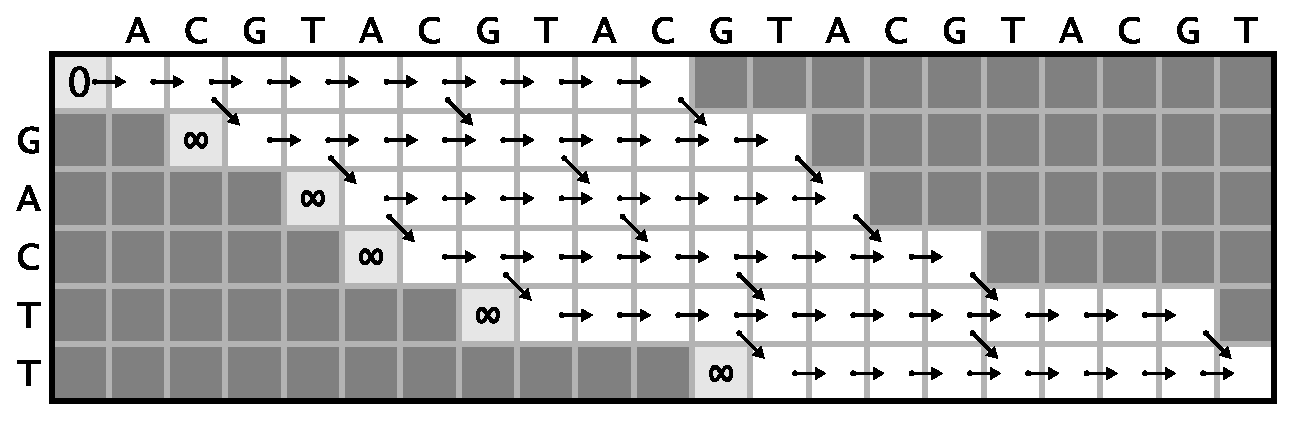
\includegraphics[width=\textwidth]{reembed/ospe}
\caption{\label{fig:ospe}%
  OSPE's dynamic programming matrix for computing an optimal embedding of a
  probe $p=\text{GACTT}$ in a deposition sequence $N=\text{\{ACGT\}}^5$. Dark
  shaded cells are not computed. Arrows show all paths in the matrix leading to
  a valid embedding of $p$ in $N$.}
\end{figure}

Once $D$ is computed, the minimum cost is $D[\ell,T]$, and an optimal embedding
of $p$ in $N$ can be constructed by tracing a path from $D[\ell,T]$ back to
$D[0,0]$, similarly to the procedure used to build an optimal global alignment.
This takes $O(T)$ time.

The OSPE algorithm is the basic operation of several post-placement optimization
algorithms: Chessboard, Greedy and Batched Greedy, Sequential as well as our new
Priority re-embedding algorithm. The main difference between these algorithms
lies in the order in which the probes are re-embedded.

Since OSPE never increases the amount of conflicts in the region around the
re-embedded probe, optimization algorithms can execute several re-embedding
operations without risk of worsening the current layout. Moreover, each probe
may be re-embedded several times since new improvements may be possible once its
neighbors have been changed. In fact, all algorithms presented here work in
repeating cycles of optimization until no more improvements are possible (when a
local optimal solution is found), until improvements drop below a given
threshold $W$, or until a given number of cycles (or \emph{passes}) have been
executed.

%%%%%%%%%%%%%%%%%%%%%%%%%%%%%%%%%%%%%%%%%%%%%%%%%%%%%%%%%%%%%%%%%%%%%%%%%%%%%%%%
\section{Chessboard}
\label{sec:reembed_chessboard}

The Chessboard re-embedding algorithm \citep{Kahng2002} was initially designed
for border length minimization, and it takes advantage of the fact that, in this
model, a chip can be bi-colored like a chessboard, in such a way that the
embeddings of probes located on white spots are independent of those placed on
black spots (Fig.~\ref{fig:chessboard}a).

Chessboard uses this coloring to alternate the optimal re-embedding of probes
located on black and white spots with respect to their neighbors: Each pass of
Chessboard consists of re-embedding all probes of black spots and then all probe
of white spots.

The chessboard coloring guarantees that probes re-embedded in the same step are
independent with respect to the border length model, i.e. they can be
re-embedded without affecting the border conflicts of other spots with the same
color. For conflict index minimization, the same principle can be applied by
using $4\times 4=16$ colors instead of~$2$ as illustrated in
Fig.~\ref{fig:chessboard} (to our knowledge this has not yet been implemented).

\begin{figure}[t]\centering
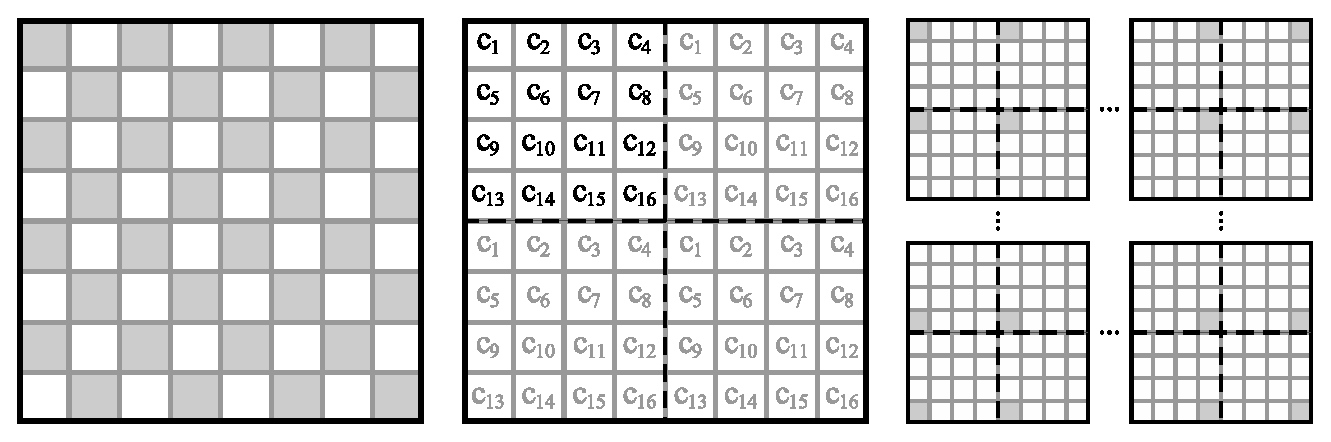
\includegraphics[width=\textwidth]{reembed/chessboard}
\begin{picture}(435,20)
\put(-3,0){ \makebox(136,20){a)}}
\put(150,0){\makebox(137,20){b)}}
\put(301,0){\makebox(136,20){c)}}
\end{picture}
\caption{\label{fig:chessboard}%
  a) The chessboard-like bi-coloring of a chip used by the Chessboard
  re-embedding algorithm for border length minimization; b) a possible coloring
  of the chip for conflict index minimization using 16 colors
  ($c_1 \dots c_{16}$), resulting in sets of independent spots; c) four of the
  16 sets of independent spots (shaded) that can be re-embedded in the same
  iteration.}
\end{figure}

%%%%%%%%%%%%%%%%%%%%%%%%%%%%%%%%%%%%%%%%%%%%%%%%%%%%%%%%%%%%%%%%%%%%%%%%%%%%%%%%
\section{Greedy and Batched Greedy}
\label{sec:reembed_greedy}
  
As its name implies, the Greedy re-embedding algorithm \citep{Kahng2002}
utilizes a greedy strategy for choosing the order in which probes are
re-embedded. At each iteration, Greedy examines every spot of the chip and
computes the maximum reduction of border conflicts achievable by optimally
re-embedding its probe. It then selects a spot with the highest gain (reduction
of conflicts) and re-embeds its probe optimally, updating the gains of adjacent
spots.

A faster version of this algorithm, called Batched Greedy \citep{Kahng2002},
pre-selects several independent spots for re-embedding and thus sacrifices its
greedy nature in favour of running time by postponing the update of gains.

Like Chessboard, Greedy and Batched Greedy were initially developed for border
length minmization, but they can also be extended for conflict index
minimization. The main difference is that, once a probe is re-embedded, more
neighbors need to be updated. For Batched Greedy, the selection of independent
spots need to take into account the minimum distance of four cells (horizonally
and vertically) between spots, in accordance with the conflict index model
(Sect.~\ref{sec:mlp_conflict_index}). Hence fewer spots may be be re-embedded in
the same iteration.

%%%%%%%%%%%%%%%%%%%%%%%%%%%%%%%%%%%%%%%%%%%%%%%%%%%%%%%%%%%%%%%%%%%%%%%%%%%%%%%%
\section{Sequential re-embedding}
\label{sec:reembed_sequential}

The Sequential algorithm \citep{Kahng2003a} employs a much simpler and,
surprisingly, more efficient strategy. The algorithm just proceeds spot by spot,
from top to bottom, left to right, re-embedding each probe optimally in regards
to its neighbors. Once the end of the array is reached, Sequential restarts at
the top left of the array for the next iteration.

The algorithm is not only simple but also fast since there is no need to compute
achievable gains for each spot. Nonetheless, Sequential achieved the greatest
reduction of border conflicts in the experiments of \citet{Kahng2003a}. The
authors argue that the main shortcoming of Chessboard and Greedy is that they
always re-embed an independent set of spots at a time, and dropping this
requirement should allow faster propagation of the effects of new embeddings and
hence convergence to a better local optimum.

Tables \ref{tab:sequential_bl} and ~\ref{tab:sequential_ci} show the results of
using Sequential to re-embed the probes of chips produced by the Greedy
placement algorithm (Sect.~\ref{sec:placement_greedy}). The chips initially
contained random probes of length 25, uniformly generated, and left-most
embedded in the standard Affymetrix deposition sequence.
The threshold $W$ was set to $0.2\%$ (Sequential stopped as soon as the total
reduction of conflicts in one pass droped below $0.2\%$). In all cases, the
threshold was reached after two passes.

\begin{table}[t]\centering
\caption{\label{tab:sequential_bl}
  Normalized border length (NBL) before and after an optimization phase with the
  Sequential re-embedding algorithm. Placement was produced by the Greedy
  placement algorithm (see Sect.~\ref{sec:placement_greedy}) with border length
  minimization, $0$-threading, and number $Q$ of candidates per spot set to 5K
  and 20K. The average number of passes executed by Sequential before the
  threshold $W=0.2\%$ was reached is shown. The reduction of conflicts is also
  shown in percentage. Running times are reported in seconds and all results are
  averages over a set of five chips. The time spent by Sequential is also shown
  as a percentage of the total time (placement plus re-embedding).}
\footnotesize{
\begin{tabular}{crrrlrrrrr}
\vspace{1pt}
     & \multicolumn{3}{c}{Greedy placement} & & \multicolumn{5}{c}{Sequential re-embedding} \\ \cline{2-4} \cline{6-10}
\vspace{1pt}
Dim. & $Q$ & NBL & Time & & NBL & Reduct. & Passes & Time & \%Total time \\
\hline
$300\times 300$ &  5K & 18.3182 &     98.5 & & 18.2121 & 0.579\% & 2.0 &  4.8 & 4.617\% \\
                & 20K & 18.0576 &    577.9 & & 17.9726 & 0.471\% & 2.0 &  4.8 & 0.830\% \\
\hline
$500\times 500$ &  5K & 17.5830 &    345.7 & & 17.4851 & 0.557\% & 2.0 & 12.7 & 3.538\% \\
                & 20K & 17.3554 & 1\,999.8 & & 17.2779 & 0.446\% & 2.0 & 12.6 & 0.625\% \\
\hline
$800\times 800$ &  5K & 16.9124 &    916.8 & & 16.8201 & 0.546\% & 2.0 & 32.6 & 3.437\% \\
                & 20K & 16.6980 & 5\,749.7 & & 16.6258 & 0.432\% & 2.0 & 32.4 & 0.560\% \\
\hline
\end{tabular}}
\end{table}

\begin{table}[ht]\centering
\caption{\label{tab:sequential_ci}
  Average conflict index (ACI) before and after an optimization phase with the
  Sequential re-embedding algorithm with $W=0.2\%$. Placement was produced by
  the Greedy placement algorithm with conflict index minimization,
  $0$-threading, and $Q$ set to 5K and 20K.}
\footnotesize{
\begin{tabular}{crrrlrrrrr}
\vspace{1pt}
     & \multicolumn{3}{c}{Greedy placement} & & \multicolumn{5}{c}{Sequential re-embedding} \\ \cline{2-4} \cline{6-10}
\vspace{1pt}
Dim. & $Q$ & ACI & Time & & ACI & Reduct. & Passes & Time & \%Total time \\
\hline
$300\times 300$ &  5K & 440.5166 &     322.4 & & 436.8630 & 0.829\% & 2.0 &    188.9 & 36.944\% \\
                & 20K & 415.5003 &  1\,818.6 & & 412.5536 & 0.709\% & 2.0 &    189.9 &  9.457\% \\
\hline
$500\times 500$ &  5K & 432.3023 &     952.5 & & 428.7410 & 0.824\% & 2.0 &    527.3 & 35.632\% \\
                & 20K & 401.4609 &  4\,027.2 & & 398.6096 & 0.710\% & 2.0 &    528.3 & 11.597\% \\
\hline
$800\times 800$ &  5K & 426.0757 &  2\,512.1 & & 422.6277 & 0.809\% & 2.0 & 1\,357.9 & 35.087\% \\
                & 20K & 392.1786 & 11\,182.8 & & 389.3929 & 0.710\% & 2.0 & 1\,352.5 & 10.790\% \\
\hline
\end{tabular}}
\end{table}

The reduction of conflicts achieved by Sequential were small (at most $0.579\%$
with border length and $0.829\%$ for CIM), which shows that there is little room
for improvements once the placement is fixed. In fact, the more time is spent
during placement (greater $Q$), the less reduction of conflicts is achieved by
re-embedding. For instance, on a $300\times 300$ chip, the reduction in average
conflict index dropped by $0.12$ percentage point (from $0.829\%$ to $0.709\%$)
when the number of candidades per spot considered by Greedy during placement was
increased from 5K to 20K.

Although the reductions of conflicts were relatively small, Sequential required
approximately half a minute to re-embedded (two times) all probes of a
$800\times 800$ chip in the BLM case, which represented about $3.44\%$ of the
aggregate time (placement and re-embedding) when $Q=5$K and only $0.56\%$ when
$Q=20$K.

In some cases, Sequential even provided comparable reduction of border
conflicts, in less time, than increasing $Q$ for Greedy. For instance, on a
$800\times 800$ chip, Greedy placement with $Q=20$K and two passes of Sequential
re-embedding produced, in approximately half of the time, a layout with only
$0.14\%$ more border conflicts than Greedy with $Q=40$K and no re-embedding
($16.6258$ NBL in $96.4$ minutes versus $16.6026$ in $189.0$ minutes,
respectively; data not shown).

Fig.~\ref{fig:sequential-bl_blm} shows the normalized border length per masking
step of a selected $500\times 500$ chip before and after a re-embedding phase
with Sequential for BLM. It is clear that the reduction of conflicts is achieved
mainly between steps 45 and 65, at the expense of a small increase in conflicts
in the final synthesis steps. This is a result of fixing the placement with
left-most embedded probes, which leaves no room for improvements in the first
masks.

In terms of CIM, the reductions were slightly higher but Sequential was over 40
times slower than in the BLM case, taking up to $36.9\%$ of the aggregate time.
This, coupled with the fact that Greedy gives significant reductions of
conflicts with increasing $Q$ even beyond 40K, makes it difficult to justify the
time spent with re-embedding, unless when $Q$ is approaching its limit (number
of probes on the chip) and one is looking for the best layout possible.

Fig.~\ref{fig:sequential-ci_blm} shows the normalized border length per masking
step of the same $500\times 500$ chip of Fig.~\ref{fig:sequential-bl_blm} before
and after a re-embedding phase with Sequential for CIM (placement was produced
by Greedy also for CIM). Again, reduction of conflicts is restricted to the
second half of synthesis steps because of the left-most embeddings, although
with relatively better improvements when compared with the border length case.

Our results also confirm that Sequential has a linear time complexity (if we
consider that each OSPE operation can be done in constant time). Sequential
performed around $19\,400$ re-embeddings per second in the BLM case and around
$475$ re-embeddings per second in the CIM case, on average.

\begin{figure}[t]\centering
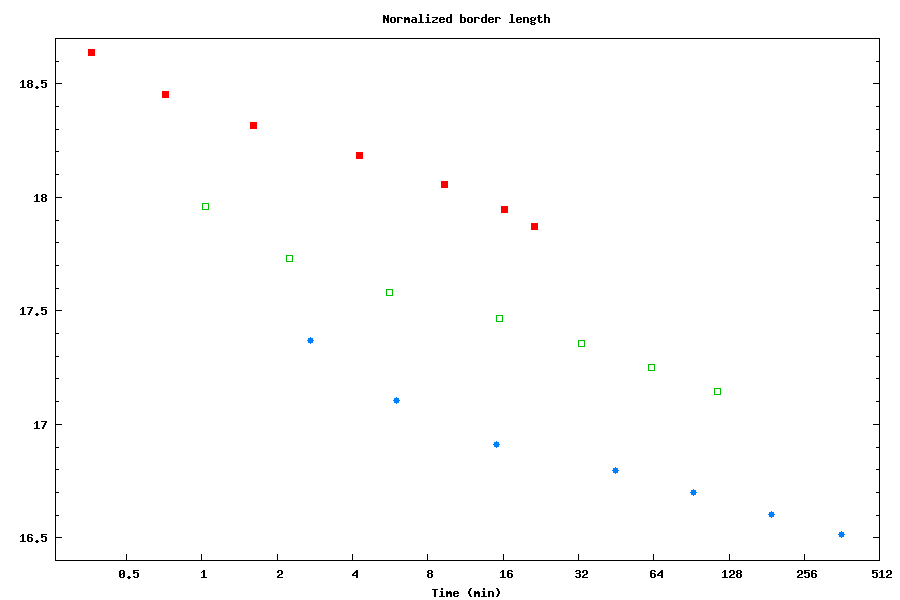
\includegraphics{reembed/sequential/bl}
\caption{\label{fig:sequential-bl_blm}
  Normalized border length per masking step of a $500\times 500$ chip before
  ({\tiny $\boxdot$}) and after ({\tiny $\times$}) a re-embedding phase with
  Sequential for border length minimization. Layout was produced by the Greedy
  placement algorithm for border length minimization with $0$-threading and
  $Q=20$K.}
\end{figure}

\begin{figure}[t]\centering
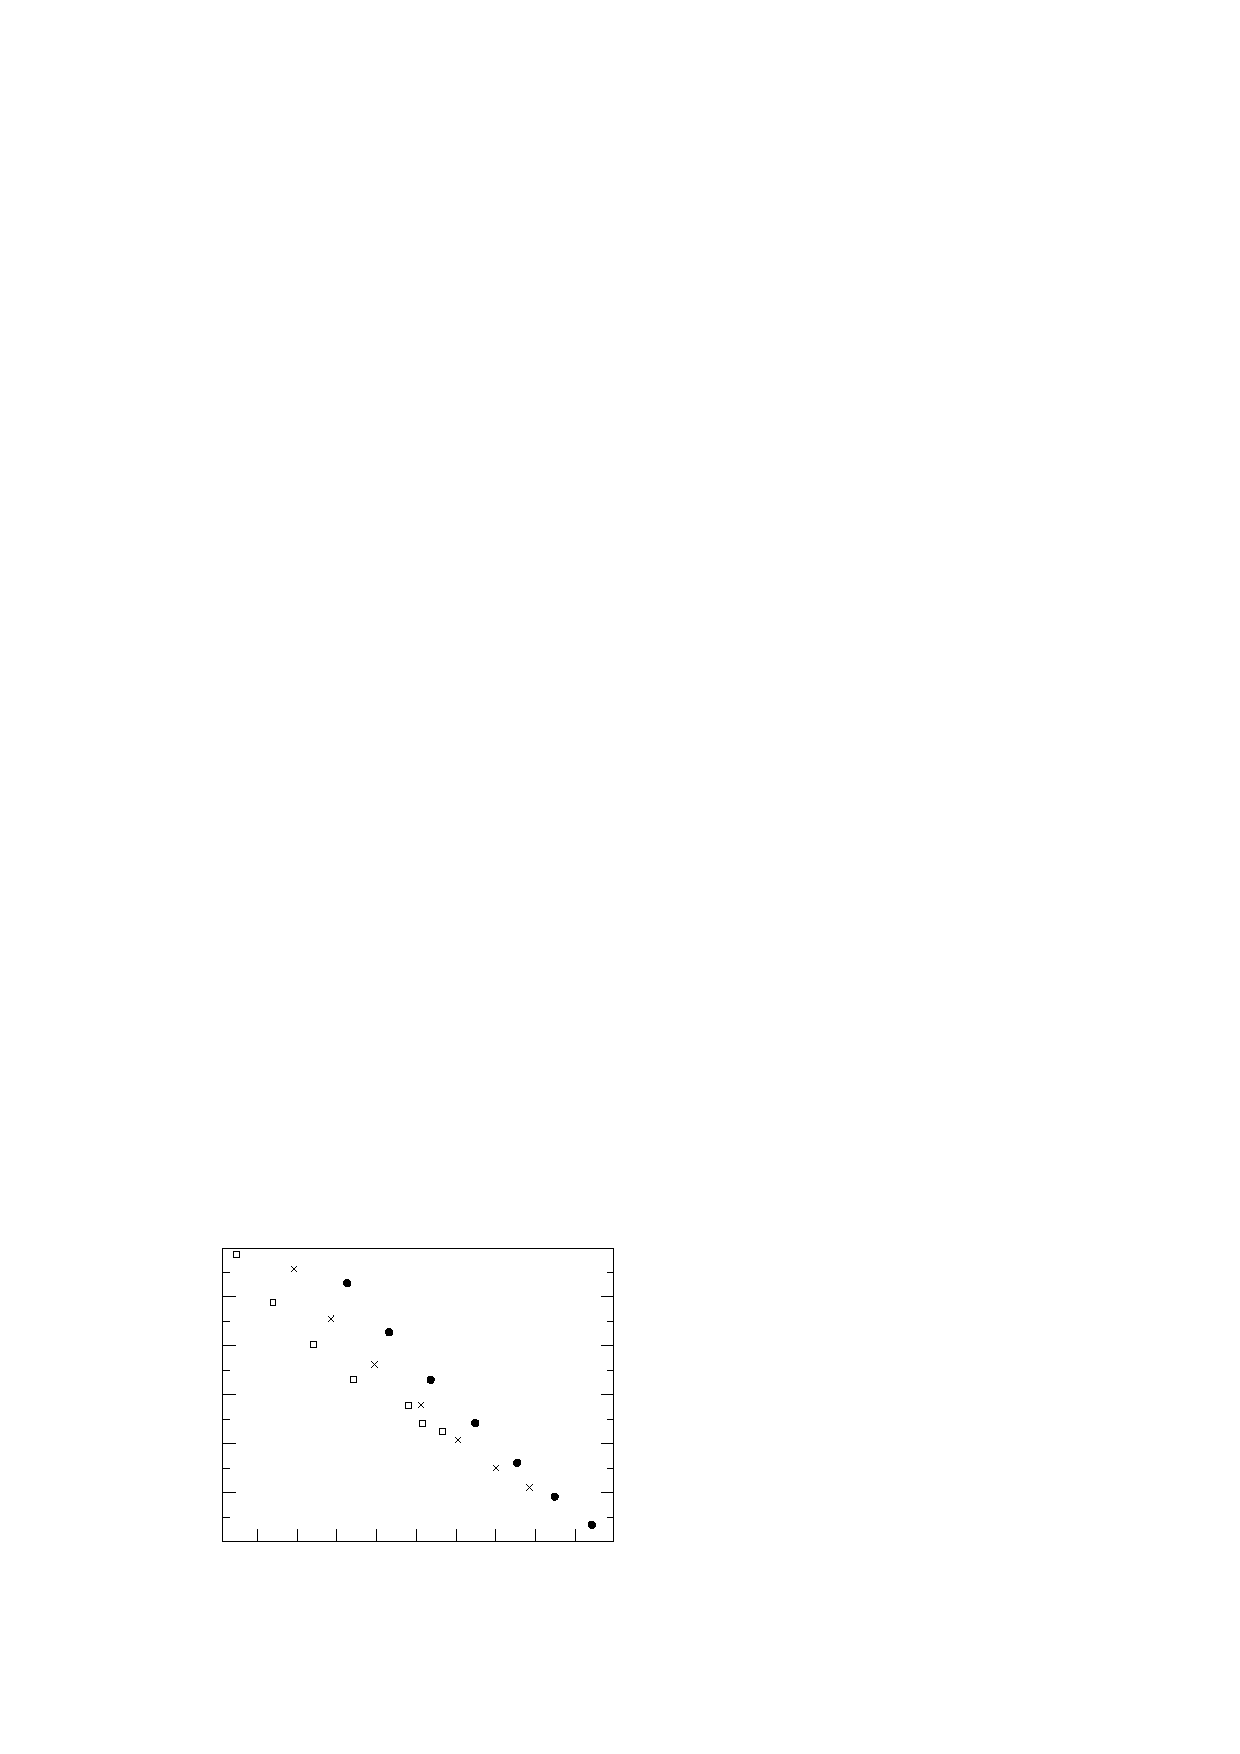
\includegraphics{reembed/sequential/ci}
\caption{\label{fig:sequential-ci_blm}
  Normalized border length per masking step of a $500\times 500$ chip before
  ({\tiny $\boxdot$}) and after ({\tiny $\times$}) a re-embedding phase with
  Sequential for conflict index minimization. Layout was produced by the Greedy
  placement algorithm for conflict index minimization with $0$-threading and
  $Q=20$K. The number of middle bases synthesized at each step is shown in boxes
  (right y-axis)}
\end{figure}

%%%%%%%%%%%%%%%%%%%%%%%%%%%%%%%%%%%%%%%%%%%%%%%%%%%%%%%%%%%%%%%%%%%%%%%%%%%%%%%%
\section{Priority re-embedding}
\label{sec:reembed_priority}

In this section we describe a new re-embedding algorithm, called Priority
re-embedding (PR), which uses a priority queue to control the order in which
probes are re-embeded.

The algorithm starts by scanning the chip for probes which have a unique
embedding in the deposition sequence. These are called \emph{pivots} and
they are used as starting locations from where the re-embeddings propagate to
other spots of the chip: Once a pivot is found, all of its four adjacent
spots on the chip are added to the priority queue. (We assume that the chip
has at least one pivot, otherwise the deposition sequence could be shortened. If
this is not the case, however, we can also use probes with the minimum number of
embeddings among all probes as pivots.)

The priority queue is used to retrieve the next spot $s$ whose probe $p$ should
be re-embedded, according to the defined priority. Once a probe $p$ is
retrieved, it is optimally re-embedded in regards to its neighbors, and all four
spots adjacent to $s$ are added to the queue (if they have not been added
previously).

We have implemented two different priorities: one based on the number of
embeddings of each probe, and one based on the number re-embedded neighbors.

\paragraph{Priority I:} Re-embed probes with fewer embeddings first.

The argument behind this priority is based on the observation that probes with
more possible embeddings have a greater degree of freedom and can more easily
``adapt'' to its neighbors. Probes with a restricted number of embeddings, on
the other hand, have less choices and should be re-embedded first.

\paragraph{Priority II:} Re-embed probes with greater number of re-embedded
neighbors first.

This priority tries to mimic the \emph{seeded crystal growth} used by the
Epitaxial placement algorithm (Sect.~\ref{sec:placement_epitaxial}), giving
preference to probes with a greater number of re-embedded neighbors. The
argument behind this priority is that probes should not be re-embedded until a
sufficient number of its neighbors have found their final embeddings.

With this priority, we assign a weight $w(s)$ for each spot $s$ in the queue,
and the spot with the highest weight is retrieved. In case of border length
minimization, $w(s)$ is set to the the number of immediate neighbors of $s$ that
have already been re-embedded in the current iteration.

In case of conflict index minimization, the algorithm looks at all 48 neighbors
in the $7\times 7$ region centered around $s$, and assigns a weight taking into
account the distance-dependent function $\gamma$ (see Eq.~\ref{eq:dist_weight}):
\[
w(s) := \sum_{\substack{s'\text{: neighbor}\\\text{of } s}}
        \Ind{s'\text{ has been re-embedded}}
        \cdot \gamma(s,s'),
\]
%%
where $s'$ ranges over all neighboring spots that are at most three cells away
(horizontally and vertically) from $s$, in accordance with the conflict index
model (Sec.~\ref{sec:mlp_conflict_index}).

With Priority II, once a probe is re-embedded, it is necessary to update the
weights of its neighbors that habe been previously added to the queue (up to 4
with border length minimization, and 48 with conflict index minimization).

\subsection{Results}

Tables \ref{tab:priority_bl} and \ref{tab:priority_ci} shows the results of
using Priority re-embedding on the same set of arrays used for Sequential
(Tables \ref{tab:sequential_bl} and \ref{tab:sequential_ci}). In terms of BLM,
both priorites resulted in negligible improvements when compared to Sequential
(with Priority I giving the best results). The greatest difference was only
$0.0032\%$ (from $18.2121$ with Sequential to $18.2115$ with Priority I on
$300\times 300$ chips and Greedy placement with $Q=5$K). Moreover, Priority I
was between $8.8\%$ and $12.7\%$ slower than Sequential, whereas Priority II was
between 2 to 5 times slower than Sequential.

Priority II is slower than Priority I because after it re-embeds a spot $s$, it
needs to update the weights of all neighbors of $s$ that have been previously
added to the queue. With Priority I, the nuber of embeddings of each probe does
not change, so they are computed only once, before the first iteration.

In terms of CIM, Priority I produced the worse layouts, whereas Priority II once
again achieved negligible improvements when compared to Sequential --- at most
$0.0029\%$ (from $412.5536$ to $412.5418$ on $300\times 300$ chips and Greedy
placement with $Q=20$K). The difference in running times between Sequential and
Priority dropped in comparison with the same difference in the BLM case. This is
because OSPE is significantly slower with CIM, so the extra time spent
re-embedding probes reduces the impact of the extra work with the priority
queue. For this reason, Priority I was always within $0.1\%$ of the time
required by Sequential, whereas Priority II was at most $11.37\%$ slower.

\begin{table}[t]\centering
\caption{\label{tab:priority_bl}
  Normalized border length (NBL) before and after an optimization phase with
  various re-embedding algorithms. Placement was produced by the Greedy
  placement algorithm with border length minimization, $0$-threading, and number
  $Q$ of candidates per spot set to 5K and 20K. In all cases, each re-embedding
  algorithm executed two passes before the threshold $W=0.2\%$ was reached. Best
  results are highlighted in bold.}
\footnotesize{
\begin{tabular}{crrlrrlrrlrr}
\vspace{1pt}
     & \multicolumn{2}{c}{Greedy placement} & & \multicolumn{2}{c}{Sequential} & & \multicolumn{2}{c}{Priority I} & & \multicolumn{2}{c}{Priority II} \\ \cline{2-3} \cline{5-6} \cline{8-9} \cline{11-12}
\vspace{1pt}
Dim. & $Q$ & NBL & & NBL & Time & & NBL & Time & & NBL & Time \\
\hline
$300\times 300$ &  5K & 18.3182 &  & 18.2121 &  4.8 &  & {\bf 18.2115} &  5.4 &  & 18.2118 &  22.0 \\
                & 20K & 18.0576 &  & 17.9726 &  4.8 &  & {\bf 17.9721} &  5.4 &  & 17.9723 &  14.5 \\
\hline
$500\times 500$ &  5K & 17.5830 &  & 17.4851 & 12.7 &  & {\bf 17.4848} & 13.9 &  & 17.4849 &  76.7 \\
                & 20K & 17.3554 &  & 17.2779 & 12.6 &  & {\bf 17.2776} & 13.7 &  & 17.2777 &  63.9 \\
\hline
$800\times 800$ &  5K & 16.9124 &  & 16.8201 & 32.6 &  & {\bf 16.8198} & 36.1 &  & 16.8199 & 187.0 \\
                & 20K & 16.6980 &  & 16.6258 & 32.4 &  & {\bf 16.6256} & 35.3 &  & 16.6257 & 200.0 \\
\hline
\end{tabular}}
\end{table}

\begin{table}[t]\centering
\caption{\label{tab:priority_ci}
  Average conflict index (ACI) before and after an optimization phase with
  various re-embedding algorithms. Placement was produced by the Greedy
  placement algorithm with conflict index minimization, $0$-threading, and number
  $Q$ of candidates per spot set to 5K and 20K. In all cases, each re-embedding
  algorithm executed two passes before the threshold $W=0.2\%$ was reached. Best
  results are highlighted in bold.}
\footnotesize{
\begin{tabular}{crrlrrlrrlrr}
\vspace{1pt}
     & \multicolumn{2}{c}{Greedy placement} & & \multicolumn{2}{c}{Sequential} & & \multicolumn{2}{c}{Priority I} & & \multicolumn{2}{c}{Priority II} \\ \cline{2-3} \cline{5-6} \cline{8-9} \cline{11-12}
\vspace{1pt}
Dim. & $Q$ & NBL & & NBL & Time & & NBL & Time & & NBL & Time \\
\hline
$300^2$ &  5K & 440.5166 &  & 436.8630 &  188.9 &  & 436.8881 &  190.7 &  & {\bf 436.8626} &  209.0 \\
                & 20K & 415.5003 &  & 412.5536 &  189.9 &  & 412.5613 &  190.0 &  & {\bf 412.5418} &  205.1 \\
\hline
$500^2$ &  5K & 432.3023 &  & 428.7410 &  527.3 &  & 428.7640 &  527.2 &  & {\bf 428.7375} &  581.6 \\
                & 20K & 401.4609 &  & 398.6096 &  528.3 &  & 398.6261 &  530.0 &  & {\bf 398.6065} &  569.5 \\
\hline
$800^2$ &  5K & 426.0757 &  & 422.6277 & 1357.9 &  & 422.6478 & 1357.9 &  & {\bf 422.6223} & 1512.2 \\
                & 20K & 392.1786 &  & 389.3929 & 1352.5 &  & 389.4075 & 1355.3 &  & {\bf 389.3903} & 1488.9 \\
\hline
\end{tabular}}
\end{table}

%%%%%%%%%%%%%%%%%%%%%%%%%%%%%%%%%%%%%%%%%%%%%%%%%%%%%%%%%%%%%%%%%%%%%%%%%%%%%%%%
\section{Summary}
\label{sec:reembed_summary}

In this chapter, we have presented an extension of the Optimum Single Probe
Embedding algorithm (OSPE) of \citet{Kahng2002} that is general enough to work
with border length as well as conflict index minimization. We have also surveyed
re-embeddings algorithms based on OSPE and presented experimental results with
Sequential, the best known algorithm to date.

In our results, it is evident that there is little room for improvements by
re-embedding probes once a placement is fixed. Nonetheless, we have also
introduced a new re-embedding algorithm that attempts to obtain better results
by changing the order of re-embeddings based on priorities. We have experimented
with two priorities: probes with fewer embeddings first (Priority I) and probes
with more re-embedded neighbors (Priority II).

Our results show that our algorithm can achive negligible improvements when
compared to Sequential, with Priority I being the best for BLM and Priority II
the best for CIM. However, because of the extra time required by Priority,
Sequential offers a better trade-off between solution quality and running time,
and it should still be the algorithm of choice unless when time is not
constrained. The results with our new algorithm also give further indication
that the improvements achievable in the re-embedding phase are rather small.
